\documentclass[twoside]{book}

% Packages required by doxygen
\usepackage{fixltx2e}
\usepackage{calc}
\usepackage{doxygen}
\usepackage[export]{adjustbox} % also loads graphicx
\usepackage{graphicx}
\usepackage[utf8]{inputenc}
\usepackage{makeidx}
\usepackage{multicol}
\usepackage{multirow}
\PassOptionsToPackage{warn}{textcomp}
\usepackage{textcomp}
\usepackage[nointegrals]{wasysym}
\usepackage[table]{xcolor}

% Font selection
\usepackage[T1]{fontenc}
\usepackage[scaled=.90]{helvet}
\usepackage{courier}
\usepackage{amssymb}
\usepackage{sectsty}
\renewcommand{\familydefault}{\sfdefault}
\allsectionsfont{%
  \fontseries{bc}\selectfont%
  \color{darkgray}%
}
\renewcommand{\DoxyLabelFont}{%
  \fontseries{bc}\selectfont%
  \color{darkgray}%
}
\newcommand{\+}{\discretionary{\mbox{\scriptsize$\hookleftarrow$}}{}{}}

% Page & text layout
\usepackage{geometry}
\geometry{%
  a4paper,%
  top=2.5cm,%
  bottom=2.5cm,%
  left=2.5cm,%
  right=2.5cm%
}
\tolerance=750
\hfuzz=15pt
\hbadness=750
\setlength{\emergencystretch}{15pt}
\setlength{\parindent}{0cm}
\setlength{\parskip}{3ex plus 2ex minus 2ex}
\makeatletter
\renewcommand{\paragraph}{%
  \@startsection{paragraph}{4}{0ex}{-1.0ex}{1.0ex}{%
    \normalfont\normalsize\bfseries\SS@parafont%
  }%
}
\renewcommand{\subparagraph}{%
  \@startsection{subparagraph}{5}{0ex}{-1.0ex}{1.0ex}{%
    \normalfont\normalsize\bfseries\SS@subparafont%
  }%
}
\makeatother

% Headers & footers
\usepackage{fancyhdr}
\pagestyle{fancyplain}
\fancyhead[LE]{\fancyplain{}{\bfseries\thepage}}
\fancyhead[CE]{\fancyplain{}{}}
\fancyhead[RE]{\fancyplain{}{\bfseries\leftmark}}
\fancyhead[LO]{\fancyplain{}{\bfseries\rightmark}}
\fancyhead[CO]{\fancyplain{}{}}
\fancyhead[RO]{\fancyplain{}{\bfseries\thepage}}
\fancyfoot[LE]{\fancyplain{}{}}
\fancyfoot[CE]{\fancyplain{}{}}
\fancyfoot[RE]{\fancyplain{}{\bfseries\scriptsize Generated by Doxygen }}
\fancyfoot[LO]{\fancyplain{}{\bfseries\scriptsize Generated by Doxygen }}
\fancyfoot[CO]{\fancyplain{}{}}
\fancyfoot[RO]{\fancyplain{}{}}
\renewcommand{\footrulewidth}{0.4pt}
\renewcommand{\chaptermark}[1]{%
  \markboth{#1}{}%
}
\renewcommand{\sectionmark}[1]{%
  \markright{\thesection\ #1}%
}

% Indices & bibliography
\usepackage{natbib}
\usepackage[titles]{tocloft}
\setcounter{tocdepth}{3}
\setcounter{secnumdepth}{5}
\makeindex

% Hyperlinks (required, but should be loaded last)
\usepackage{ifpdf}
\ifpdf
  \usepackage[pdftex,pagebackref=true]{hyperref}
\else
  \usepackage[ps2pdf,pagebackref=true]{hyperref}
\fi
\hypersetup{%
  colorlinks=true,%
  linkcolor=blue,%
  citecolor=blue,%
  unicode%
}

% Custom commands
\newcommand{\clearemptydoublepage}{%
  \newpage{\pagestyle{empty}\cleardoublepage}%
}

\usepackage{caption}
\captionsetup{labelsep=space,justification=centering,font={bf},singlelinecheck=off,skip=4pt,position=top}

%===== C O N T E N T S =====

\begin{document}

% Titlepage & ToC
\hypersetup{pageanchor=false,
             bookmarksnumbered=true,
             pdfencoding=unicode
            }
\pagenumbering{alph}
\begin{titlepage}
\vspace*{7cm}
\begin{center}%
{\Large cpp }\\
\vspace*{1cm}
{\large Generated by Doxygen 1.8.13}\\
\end{center}
\end{titlepage}
\clearemptydoublepage
\pagenumbering{roman}
\tableofcontents
\clearemptydoublepage
\pagenumbering{arabic}
\hypersetup{pageanchor=true}

%--- Begin generated contents ---
\chapter{Hierarchical Index}
\section{Class Hierarchy}
This inheritance list is sorted roughly, but not completely, alphabetically\+:\begin{DoxyCompactList}
\item \contentsline{section}{figure}{\pageref{classfigure}}{}
\begin{DoxyCompactList}
\item \contentsline{section}{disque}{\pageref{classdisque}}{}
\item \contentsline{section}{rectangle}{\pageref{classrectangle}}{}
\item \contentsline{section}{triangle}{\pageref{classtriangle}}{}
\end{DoxyCompactList}
\end{DoxyCompactList}

\chapter{Class Index}
\section{Class List}
Here are the classes, structs, unions and interfaces with brief descriptions\+:\begin{DoxyCompactList}
\item\contentsline{section}{\hyperlink{classdisque}{disque} \\*Calculer la surface et le perimetre du disque }{\pageref{classdisque}}{}
\item\contentsline{section}{\hyperlink{classfigure}{figure} \\*Fonctions perimetre et surface }{\pageref{classfigure}}{}
\item\contentsline{section}{\hyperlink{classrectangle}{rectangle} \\*Calcule du perimetre et de la surface du rectangle }{\pageref{classrectangle}}{}
\item\contentsline{section}{\hyperlink{classtriangle}{triangle} }{\pageref{classtriangle}}{}
\end{DoxyCompactList}

\chapter{File Index}
\section{File List}
Here is a list of all documented files with brief descriptions\+:\begin{DoxyCompactList}
\item\contentsline{section}{/home/epsi/figure/src/{\bfseries disque.\+h} }{\pageref{disque_8h}}{}
\item\contentsline{section}{/home/epsi/figure/src/\hyperlink{figure_8h}{figure.\+h} \\*Creation de la figure }{\pageref{figure_8h}}{}
\item\contentsline{section}{/home/epsi/figure/src/\hyperlink{rectangle_8h}{rectangle.\+h} \\*Calcul du perimetre et de la surface du rectangle }{\pageref{rectangle_8h}}{}
\item\contentsline{section}{/home/epsi/figure/src/{\bfseries triangle.\+h} }{\pageref{triangle_8h}}{}
\end{DoxyCompactList}

\chapter{Class Documentation}
\hypertarget{classdisque}{}\section{disque Class Reference}
\label{classdisque}\index{disque@{disque}}


calculer la surface et le perimetre du disque  




{\ttfamily \#include $<$disque.\+h$>$}



Inheritance diagram for disque\+:
\nopagebreak
\begin{figure}[H]
\begin{center}
\leavevmode
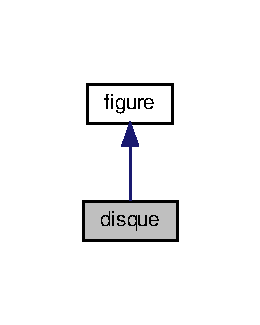
\includegraphics[width=125pt]{classdisque__inherit__graph}
\end{center}
\end{figure}


Collaboration diagram for disque\+:
\nopagebreak
\begin{figure}[H]
\begin{center}
\leavevmode
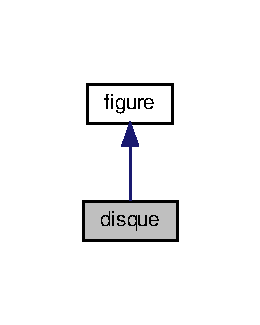
\includegraphics[width=125pt]{classdisque__coll__graph}
\end{center}
\end{figure}
\subsection*{Public Member Functions}
\begin{DoxyCompactItemize}
\item 
int \hyperlink{classdisque_a48361c6c20641c3da6db79b05e8facd6}{perimetre} (int rayon)
\item 
int \hyperlink{classdisque_a24cfaf289fe88cfcf71e3968edbd9bf4}{surface} (int rayon)
\end{DoxyCompactItemize}


\subsection{Detailed Description}
calculer la surface et le perimetre du disque 

\subsection{Member Function Documentation}
\mbox{\Hypertarget{classdisque_a48361c6c20641c3da6db79b05e8facd6}\label{classdisque_a48361c6c20641c3da6db79b05e8facd6}} 
\index{disque@{disque}!perimetre@{perimetre}}
\index{perimetre@{perimetre}!disque@{disque}}
\subsubsection{\texorpdfstring{perimetre()}{perimetre()}}
{\footnotesize\ttfamily int disque\+::perimetre (\begin{DoxyParamCaption}\item[{int}]{rayon }\end{DoxyParamCaption})}


\begin{DoxyParams}{Parameters}
{\em rayon} & calculer le perimetre avec le rayon et pi \\
\hline
\end{DoxyParams}
\mbox{\Hypertarget{classdisque_a24cfaf289fe88cfcf71e3968edbd9bf4}\label{classdisque_a24cfaf289fe88cfcf71e3968edbd9bf4}} 
\index{disque@{disque}!surface@{surface}}
\index{surface@{surface}!disque@{disque}}
\subsubsection{\texorpdfstring{surface()}{surface()}}
{\footnotesize\ttfamily int disque\+::surface (\begin{DoxyParamCaption}\item[{int}]{rayon }\end{DoxyParamCaption})}


\begin{DoxyParams}{Parameters}
{\em rayon} & calculer la surface avec le rayon et pi \\
\hline
\end{DoxyParams}


The documentation for this class was generated from the following files\+:\begin{DoxyCompactItemize}
\item 
/home/epsi/figure/src/disque.\+h\item 
/home/epsi/figure/src/disque.\+cpp\end{DoxyCompactItemize}

\hypertarget{classfigure}{}\section{figure Class Reference}
\label{classfigure}\index{figure@{figure}}


fonctions perimetre et surface  




{\ttfamily \#include $<$figure.\+h$>$}



Inheritance diagram for figure\+:
\nopagebreak
\begin{figure}[H]
\begin{center}
\leavevmode
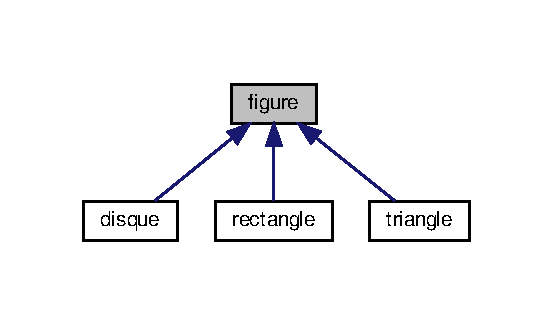
\includegraphics[width=266pt]{classfigure__inherit__graph}
\end{center}
\end{figure}
\subsection*{Public Member Functions}
\begin{DoxyCompactItemize}
\item 
\mbox{\Hypertarget{classfigure_a6ad51de31732e21f412ee7482e688ed0}\label{classfigure_a6ad51de31732e21f412ee7482e688ed0}} 
int {\bfseries perimetre} ()
\item 
\mbox{\Hypertarget{classfigure_a4ab3ef3c25af52a19979f5824fb790da}\label{classfigure_a4ab3ef3c25af52a19979f5824fb790da}} 
int {\bfseries surface} ()
\end{DoxyCompactItemize}


\subsection{Detailed Description}
fonctions perimetre et surface 

The documentation for this class was generated from the following files\+:\begin{DoxyCompactItemize}
\item 
/home/epsi/figure/src/\hyperlink{figure_8h}{figure.\+h}\item 
/home/epsi/figure/src/figure.\+cpp\end{DoxyCompactItemize}

\hypertarget{classrectangle}{}\section{rectangle Class Reference}
\label{classrectangle}\index{rectangle@{rectangle}}


calcule du perimetre et de la surface du rectangle  




{\ttfamily \#include $<$rectangle.\+h$>$}



Inheritance diagram for rectangle\+:
\nopagebreak
\begin{figure}[H]
\begin{center}
\leavevmode
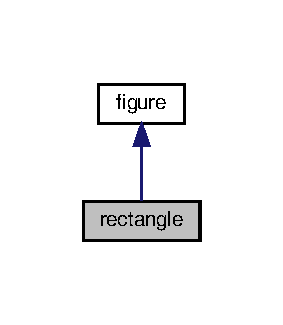
\includegraphics[width=136pt]{classrectangle__inherit__graph}
\end{center}
\end{figure}


Collaboration diagram for rectangle\+:
\nopagebreak
\begin{figure}[H]
\begin{center}
\leavevmode
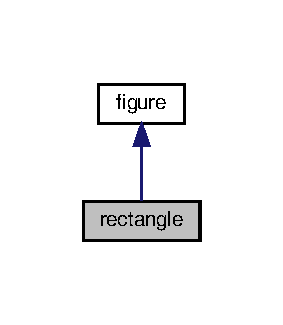
\includegraphics[width=136pt]{classrectangle__coll__graph}
\end{center}
\end{figure}
\subsection*{Public Member Functions}
\begin{DoxyCompactItemize}
\item 
int \hyperlink{classrectangle_aa613ad02ccb6dac181af4da6582315e6}{perimetre} (int longueur, int largeur)
\item 
int \hyperlink{classrectangle_a5923870fc20835f463cde0f64023b042}{surface} (int longueur, int largeur)
\end{DoxyCompactItemize}


\subsection{Detailed Description}
calcule du perimetre et de la surface du rectangle 

\subsection{Member Function Documentation}
\mbox{\Hypertarget{classrectangle_aa613ad02ccb6dac181af4da6582315e6}\label{classrectangle_aa613ad02ccb6dac181af4da6582315e6}} 
\index{rectangle@{rectangle}!perimetre@{perimetre}}
\index{perimetre@{perimetre}!rectangle@{rectangle}}
\subsubsection{\texorpdfstring{perimetre()}{perimetre()}}
{\footnotesize\ttfamily int rectangle\+::perimetre (\begin{DoxyParamCaption}\item[{int}]{longueur,  }\item[{int}]{largeur }\end{DoxyParamCaption})}


\begin{DoxyParams}{Parameters}
{\em longueur} & \\
\hline
{\em largeur} & \\
\hline
\end{DoxyParams}
\mbox{\Hypertarget{classrectangle_a5923870fc20835f463cde0f64023b042}\label{classrectangle_a5923870fc20835f463cde0f64023b042}} 
\index{rectangle@{rectangle}!surface@{surface}}
\index{surface@{surface}!rectangle@{rectangle}}
\subsubsection{\texorpdfstring{surface()}{surface()}}
{\footnotesize\ttfamily int rectangle\+::surface (\begin{DoxyParamCaption}\item[{int}]{longueur,  }\item[{int}]{largeur }\end{DoxyParamCaption})}


\begin{DoxyParams}{Parameters}
{\em longueur} & \\
\hline
{\em largeur} & \\
\hline
\end{DoxyParams}


The documentation for this class was generated from the following files\+:\begin{DoxyCompactItemize}
\item 
/home/epsi/figure/src/\hyperlink{rectangle_8h}{rectangle.\+h}\item 
/home/epsi/figure/src/rectangle.\+cpp\end{DoxyCompactItemize}

\hypertarget{classtriangle}{}\section{triangle Class Reference}
\label{classtriangle}\index{triangle@{triangle}}


Inheritance diagram for triangle\+:
\nopagebreak
\begin{figure}[H]
\begin{center}
\leavevmode
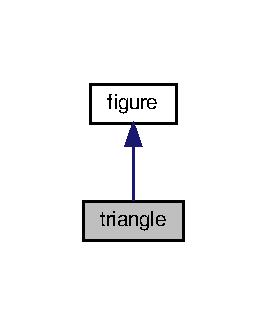
\includegraphics[width=128pt]{classtriangle__inherit__graph}
\end{center}
\end{figure}


Collaboration diagram for triangle\+:
\nopagebreak
\begin{figure}[H]
\begin{center}
\leavevmode
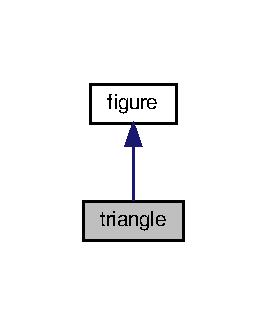
\includegraphics[width=128pt]{classtriangle__coll__graph}
\end{center}
\end{figure}
\subsection*{Public Member Functions}
\begin{DoxyCompactItemize}
\item 
\mbox{\Hypertarget{classtriangle_a4b47dbb5ecace0640ab3b3ffb4aba68f}\label{classtriangle_a4b47dbb5ecace0640ab3b3ffb4aba68f}} 
int {\bfseries perimetre} (int cote1, int cote2, int cote3)
\item 
\mbox{\Hypertarget{classtriangle_a378b6ee932d5373eb84c8a2a24e5e005}\label{classtriangle_a378b6ee932d5373eb84c8a2a24e5e005}} 
int {\bfseries surface} (int hauteur, int base)
\end{DoxyCompactItemize}


The documentation for this class was generated from the following files\+:\begin{DoxyCompactItemize}
\item 
/home/epsi/figure/src/triangle.\+h\item 
/home/epsi/figure/src/triangle.\+cpp\end{DoxyCompactItemize}

\chapter{File Documentation}
\hypertarget{figure_8h}{}\section{/home/epsi/figure/src/figure.h File Reference}
\label{figure_8h}\index{/home/epsi/figure/src/figure.\+h@{/home/epsi/figure/src/figure.\+h}}


creation de la figure  


{\ttfamily \#include $<$iostream$>$}\newline
Include dependency graph for figure.\+h\+:
\nopagebreak
\begin{figure}[H]
\begin{center}
\leavevmode
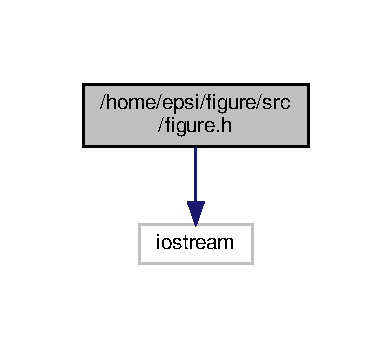
\includegraphics[width=188pt]{figure_8h__incl}
\end{center}
\end{figure}
This graph shows which files directly or indirectly include this file\+:
\nopagebreak
\begin{figure}[H]
\begin{center}
\leavevmode
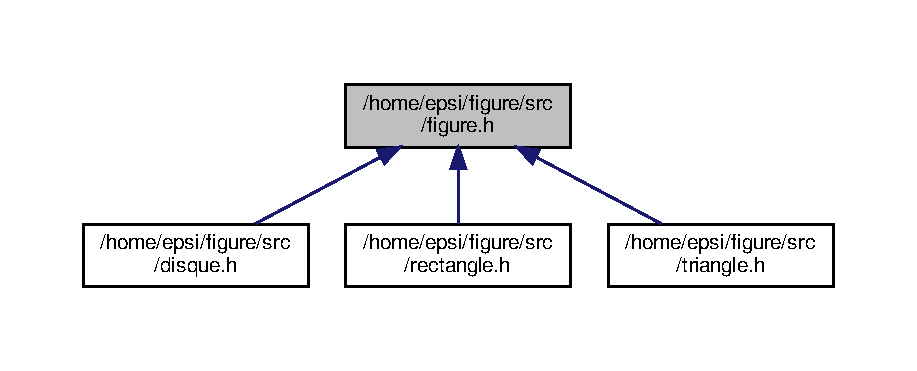
\includegraphics[width=350pt]{figure_8h__dep__incl}
\end{center}
\end{figure}
\subsection*{Classes}
\begin{DoxyCompactItemize}
\item 
class \hyperlink{classfigure}{figure}
\begin{DoxyCompactList}\small\item\em fonctions perimetre et surface \end{DoxyCompactList}\end{DoxyCompactItemize}


\subsection{Detailed Description}
creation de la figure 

\begin{DoxyAuthor}{Author}
Yohann Louisia 
\end{DoxyAuthor}
\begin{DoxyVersion}{Version}
1.\+0 
\end{DoxyVersion}

\hypertarget{rectangle_8h}{}\section{/home/epsi/figure/src/rectangle.h File Reference}
\label{rectangle_8h}\index{/home/epsi/figure/src/rectangle.\+h@{/home/epsi/figure/src/rectangle.\+h}}


calcul du perimetre et de la surface du rectangle  


{\ttfamily \#include \char`\"{}figure.\+h\char`\"{}}\newline
Include dependency graph for rectangle.\+h\+:
\nopagebreak
\begin{figure}[H]
\begin{center}
\leavevmode
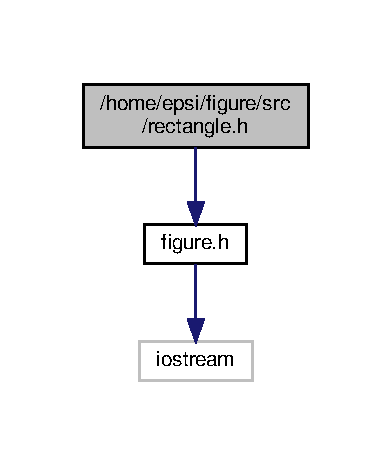
\includegraphics[width=188pt]{rectangle_8h__incl}
\end{center}
\end{figure}
\subsection*{Classes}
\begin{DoxyCompactItemize}
\item 
class \hyperlink{classrectangle}{rectangle}
\begin{DoxyCompactList}\small\item\em calcule du perimetre et de la surface du rectangle \end{DoxyCompactList}\end{DoxyCompactItemize}


\subsection{Detailed Description}
calcul du perimetre et de la surface du rectangle 

\begin{DoxyAuthor}{Author}
Yohann Louisia 
\end{DoxyAuthor}
\begin{DoxyVersion}{Version}
1.\+0 
\end{DoxyVersion}

%--- End generated contents ---

% Index
\backmatter
\newpage
\phantomsection
\clearemptydoublepage
\addcontentsline{toc}{chapter}{Index}
\printindex

\end{document}
